% Source: graduate-coursework/Sp26/CSCE775/course_notes/quiz_2_study_guide.tex

\documentclass[border=4pt]{standalone}
\usepackage{amsmath, amssymb}
\usepackage{tikz}
\usepackage{xcolor}
\usetikzlibrary{arrows.meta, positioning, calc}

\definecolor{garnet}{HTML}{73000A}
\definecolor{black90}{HTML}{363636}
\definecolor{atlantic}{HTML}{466A9F}
\definecolor{congaree}{HTML}{1F414D}
\definecolor{horseshoe}{HTML}{65780B}
\definecolor{rose}{HTML}{CC2E40}

\newcommand{\important}[1]{\textcolor{garnet}{\textbf{#1}}}
\newcommand{\concept}[1]{\textcolor{atlantic}{\textbf{#1}}}
\newcommand{\formula}[1]{\begin{center}\fcolorbox{garnet}{white}{\parbox{0.9\linewidth}{#1}}\end{center}}
\newcommand{\intuition}[1]{\begin{center}\fcolorbox{atlantic}{blue!3}{\parbox{0.9\linewidth}{\textcolor{atlantic}{\textbf{Intuition:}} #1}}\end{center}}
\newcommand{\example}[1]{\begin{center}\fcolorbox{horseshoe}{green!3}{\parbox{0.9\linewidth}{\textcolor{horseshoe}{\textbf{Example:}} #1}}\end{center}}

\begin{document}
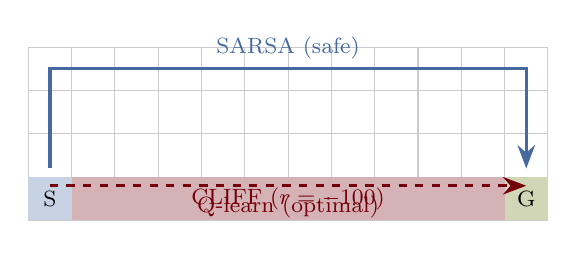
\begin{tikzpicture}[scale=0.55, every node/.style={font=\footnotesize}]
    % Grid
    \foreach \x in {0,...,11} \foreach \y in {0,...,3}
        \draw[black!20] (\x,\y) rectangle (\x+1,\y+1);
    % Cliff
    \foreach \x in {1,...,10}
        \fill[garnet!30] (\x,0) rectangle (\x+1,1);
    \node[garnet] at (6, 0.5) {CLIFF ($r = -100$)};
    % Start/Goal
    \fill[atlantic!30] (0,0) rectangle (1,1);
    \node at (0.5,0.5) {S};
    \fill[horseshoe!30] (11,0) rectangle (12,1);
    \node at (11.5,0.5) {G};
    % Paths
    \draw[-{Stealth}, atlantic, very thick] (0.5,1.2) -- (0.5,3.5) -- (11.5,3.5) -- (11.5,1.2);
    \node[atlantic, above] at (6,3.5) {SARSA (safe)};
    \draw[-{Stealth}, garnet, very thick, dashed] (0.5,0.8) -- (1,0.8) -- (11,0.8) -- (11.5,0.8);
    \node[garnet, below] at (6,0.8) {\footnotesize Q-learn (optimal)};
\end{tikzpicture}
\end{document}
